\documentclass[12pt]{article}
\setlength{\oddsidemargin}{0in}
\setlength{\evensidemargin}{0in}
\setlength{\textwidth}{6.5in}
\setlength{\parindent}{0in}
\setlength{\parskip}{\baselineskip}

\usepackage{amsmath,amsfonts,amssymb,xcolor,geometry}
\usepackage{graphicx}
\usepackage{fancyhdr}
\pagestyle{fancy}


\begin{document}

\rhead{{\bf CSCI 3104 \\Problem Set 5\\ Spring 2017, CU-Boulder}}
\lhead{{\bf 
        Sam Cuthbertson (06/16)\\ 
        Grant Baker (07/23) \\ 
        Connor Hudson (05/07)}}
\renewcommand{\headrulewidth}{0.4pt}
\headheight = 43pt

\renewcommand{\arraystretch}{1.5}

\vspace{-3mm}
\begin{enumerate}
		 
	\item \label{q:1} (50 pts total) Recall that Huffman's algorithm takes as input a vector {\tt f} of length $n$, containing the frequencies of the input symbol set $\Sigma$ and returns a Huffman encoding tree. We can make 
the process of encoding real strings faster by instead returning a ``codebook,'' which is a dictionary ADT $T$ that contains $n$ key-value pairs $(x_{i},y_{i})$, where $x_{i}\in \Sigma$ and $y_{i}$ is the Huffman binary encoding of 
$x_{i}$. Let $T(x_{i})=y_{i}$. Hence, the encoding of {\tt x} $=x_{1}x_{2}x_{3}\dots x_{\ell}$ is simply {\tt y} $=T(x_{1})T(x_{2})T(x_{3})\dots T(x_{\ell})$.\footnote{Collaboration with Luke Meszar.}

	In this problem, we will implement and apply three functions.
	
	(i) {\tt string2freq} takes as input an ASCII string {\tt x} and returns (a) a vector {\tt S}, which contains the $n$ unique symbols of {\tt x} in lexicographic order, and (b) a vector {\tt f} containing the frequencies of 
those symbols, in the same order. 
	
	(ii) {\tt huffmanEncode} takes as input the vectors {\tt S} and {\tt f}, and returns a dictionary {\tt T}, that represents the codebook.
	
	(iii) {\tt encodeString} takes an input ASCII string {\tt x} and a codebook {\tt T}, and returns a string {\tt y}, which is the binary encoding of {\tt x} using {\tt T}:

	If we then call {\tt y=encodeString( x , huffmanEncode( string2freq(x) ) )}, we can obtain an optimal prefix-free binary encoding {\tt y} of an input string {\tt x}.
	
	
	\begin{enumerate}
	\item \label{q:1:code} \textit{From scratch, implement the {\tt string2freq}, {\tt huffmanEncode}, and {\tt encodeString} functions. For Huffman's algorithm, you must use a priority queue data structure (or equivalent), in 
which {\tt insert} and {\tt deletemin} operations cost $O(\log n)$. You may not use any library that implements a priority queue (or equivalent) data structure---the goal is for you to implement it yourself, using only basic 
language features. Within the priority queue, ties should be broken uniformly at random. Submit your code implementation, with code comments.}
	
	Our code implementation is attached below in the \textbf{Code Appendix}.
		
	\item \textit{Using asymptotic analysis, determine the running time of the call \\ ${}^{}$\hspace{10mm} {\tt y=encodeString( x , huffmanEncode( string2freq(x) ) )} \\ for an input string {\tt x} where $\forall_{i}~x_{i}\in 
\Sigma$ and $|\Sigma|=n$. Justify your answer.}
	
    In our code, we have ${\tt string2freq(x)} = O(n\log n)$ based on the sorting algorithm used. {\tt huffmanEncode} uses a loop of length $n$ around a queue insert operation (giving a runtime of $O(n\log n)$), and another loop of 
length $n$ around operations which take $O(\log n)$. Then, we have ${\tt huffmanEncode( string2freq(x) )} = O(n\log n)$.\\
    
    {\tt encodeString} uses a single loop to run through the characters of {\tt x} and look them up in the codebook, giving another runtime of $n\log n$.\footnote{See the Python 3 documentation for a detailed description of the 
runtimes for the system functions we used. {\tt https://docs.python.org/3/}}\\
    
    Thus, we see that the runtime for {\tt y=encodeString( x , huffmanEncode( string2freq(x) ) )} is $O(n\log n)$.\\
	
	\item \textit{The data file for PS5 (see class Moodle) contains the text of a famous poem by Robert Frost. The text is given as a string {\tt x} containing $\ell=761$ symbols drawn from an alphabet $\Sigma$ containing 31 
ASCII symbols (24 alphabetical characters, 6 punctuation marks and 1 space character)
	A plaintext ASCII character normally takes 8 bits of space. How many bits does {\tt x} require when encoded in ASCII?}
	
	As an ASCII charater takes up 8 bits and the data file has 761 characters, the file takes up $8*761 = \boxed{6088}$ bits when stored in ASCII.
	
	
	\item \textit{\label{q:1:entropy}Claude Shannon famously proved that the lower bound on the number of encoded bits per input symbol for a prefix-free binary encoding of a string {\tt x} is given by the {\em entropy} 
function, defined as}
	\begin{align}
	H & = -\sum_{i=1}^{|\Sigma|} \left(\frac{f_{i}}{\ell}\right) \log_{2} \left(\frac{f_{i}}{\ell}\right) \label{q:H} \enspace ,
	\end{align}
	
    \textit{where $f_{i}$ is the frequency in {\tt x} of the $i$th symbol of $\Sigma$, and $\ell$ is the length of {\tt x}. Because we take $\log_{2}$, $H$ has units of ``bits.'' Using Eq.~\eqref{q:H}, compute (i) the predicted 
number of bits per symbol needed to optimally encode the Frost poem, and (ii) the predicted number of bits needed to encode the entire poem.}
    
    Using the function \texttt{findEntropy} in our attached code, we found H for the provided data file to be \boxed{\text{4.1345 bits per symbol}} with a subsequent size of encoded poem at $4.1254 * 761 = \boxed{\text{3139.4294 
bits}}$

	\item \textit{Now, encode {\tt x} using your Huffman encoder from part~\eqref{q:1:code} and report the number of bits in the encoded string. Compare this number to the lower bound obtained in part~\eqref{q:1:entropy}, and 
comment on the comparison.}
	
    Using our implementation of Huffman Encoding, our encoded string was length \boxed{3174} This is remarkably close to the lower bound of 3139. Our reasoning behind why this isn't at 3139 is that there are many ties of 
frequencies in the data file, with something like 5 different characters appearing only once. This will lead to an unbalanced encoding tree, which is suboptimal. 
		
	\end{enumerate}


    \newpage
	\item \textit{(35 pts) Here, ... Give a clear and concise description (1-2 paragraphs) of exactly how you modified your code and ran your experiment. No credit if axes or trend lines are not labeled, or if your plot is not 
on log-log axes.} \footnote{Collaboration with Luke Meszar.}
	
	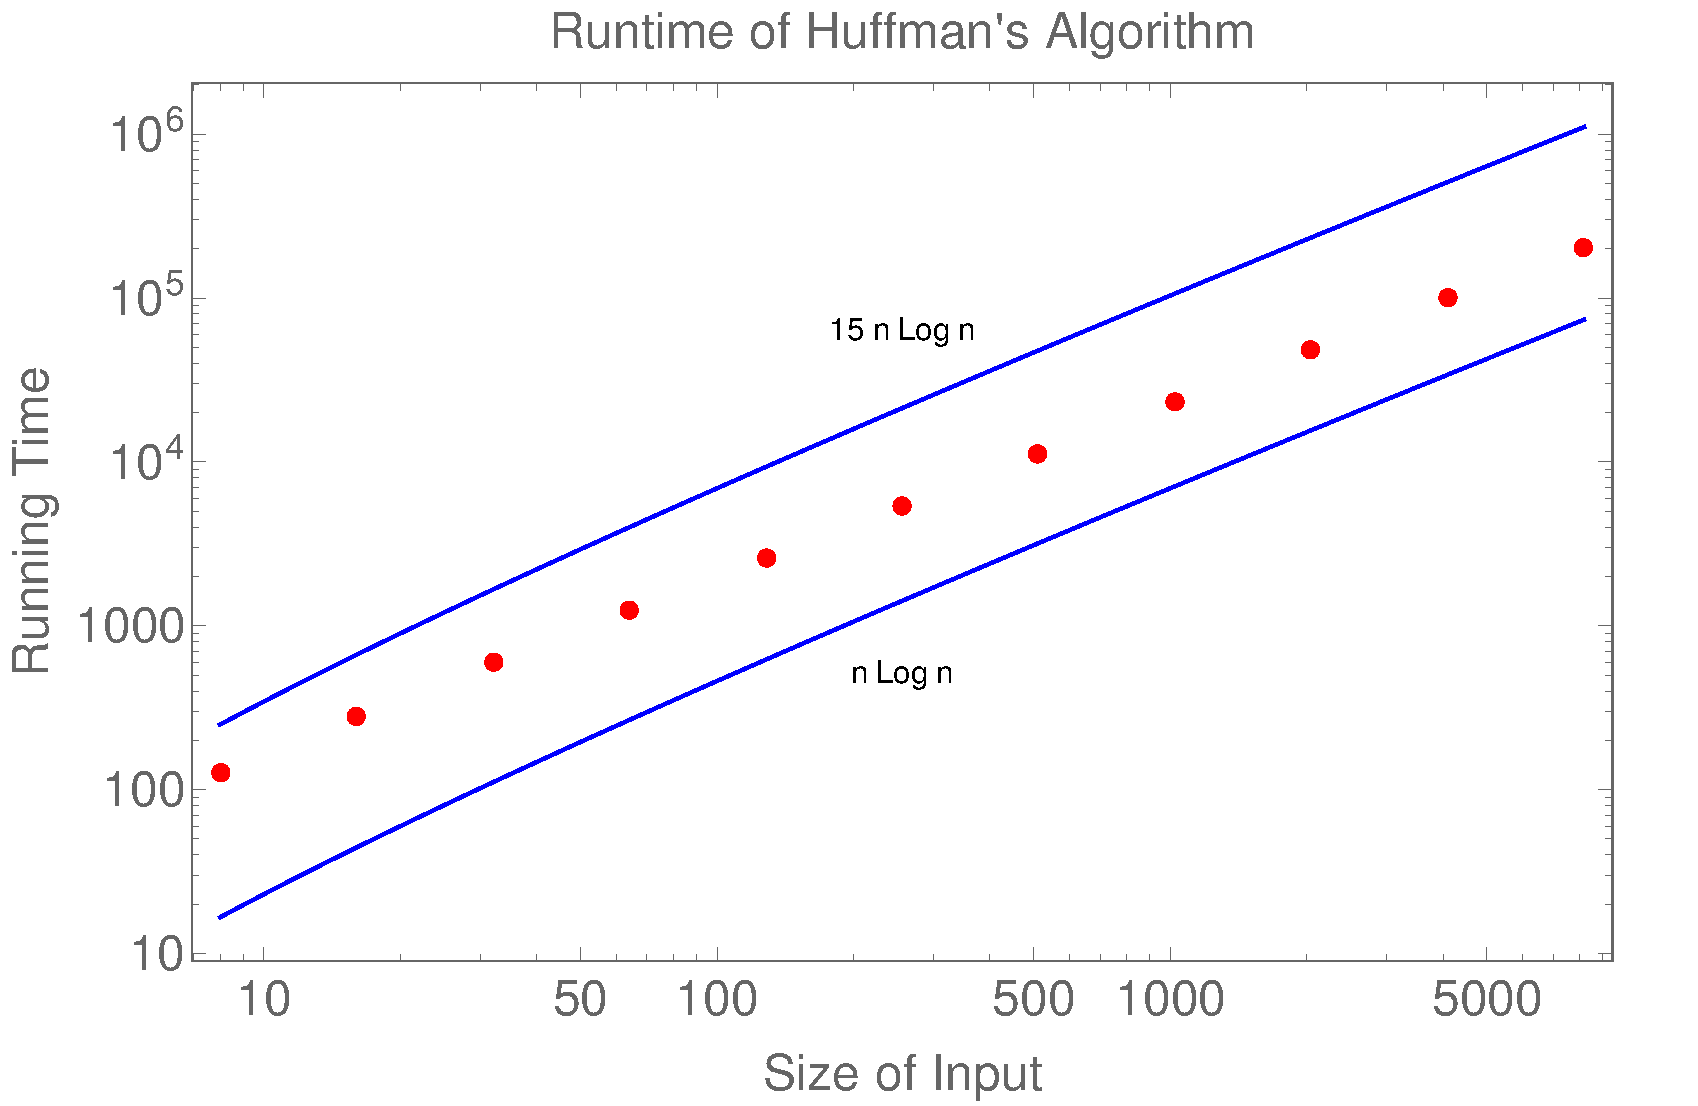
\includegraphics[width=\textwidth]{ps5p2-results}
	
    As we can see above, our {\tt huffmanEncode} function takes $\Theta(n\lg (n))$ time, bounded above by $O(n\lg (n))$ and bounded below by $\Omega(15 * n\lg (n))$. This fits our analyzed running time in 1(b), as we found our 
expected running time to be at least $O(n\lg n)$.
    
    We modified our code to increase a counter every time that a function was called or a variable was changed inside a for loop. This meant that we had counters inside {\tt addCode}, {\tt get}, {\tt put}, {\tt minUpHeapify}, {\tt 
minHeapify}, {\tt minChild} and a counter which accumulated all of those in {\tt huffmanEncode}. 
    
    We did not attach our code as it is not explicitly stated in the problem, and would significantly add to the tedium and difficulty of grading. 

	\newpage
	\item \textit{(10 pts) Ginerva Weasley is playing with the network given below. Help her calculate the number of paths from node 1 to node 14.}
	
	Note that the number of paths to 14 is equal to the below, where $P_1 = 1$:
	\begin{align*}
	    P_{14} &= P_{13} + P_{11}  &\text{Note: } &P_{13} = P_{12} + P_{10}, \; P_{11} = P_{10} + P_6\\
	           &= P_{12} + P_{10} + P_{10} + P_{6}  &&P_{12} = P_9, \; P_{10} = P_5 + P_9, \; P_6 = P_5\\
	           &= P_{9} + 2(P_5 + P_9) + P_5 &&P_5 = P_4\\
	           &= 3(P_4 + P_9) &&P_4 = P_3, \; P_9 = P_8 + P_3\\
	           &= 3(P_3 + P_3 + P_8) &&P_3 = P_2, \; P_8 = P_2 + P_7\\
	           &= 3(2(P_2) + P_2 + P_7) &&P_7 = P_2 + P_1 = P_2 + 1 \\
	           &= 3(3(P_2) + P_2 + P_2 + 1) \\
	           &= 3(5(P_2)) + 3 &&P_2 = P_1 = 1\\
	           &= 15(1) + 3 \\
	           &= \boxed{18 \text{ Paths}}
	\end{align*}
	
	
    \newpage
	\item \textit{(30 pts total) Ron and Hermione are having a competition to see who can compute the $n$th Lucas number $L_{n}$ more quickly, without resorting to magic. Recall that the $n$th Lucas number is defined as $L_{n} 
= L_{n-1} +L_{n-2}$ for $n>1$ with base cases $L_{0} =2$ and $L_{1} =1$. Ron opens with the classic recursive algorithm:}
	
	\begin{small}
	\begin{verbatim}
	Luc(n) :
	   if n == 0 { return 2 }
	   else if n == 1 { return 1 }
	   else { return Luc(n-1) + Luc(n-2) }
	\end{verbatim}
	\end{small}
	
	\textit{which he claims takes $R(n) = R(n-1) + R(n-2) + c = O(\phi^{n})$ time.}
	
	\begin{enumerate}
	\item \label{q:3:memfib} \textit{Hermione counters with a dynamic programming approach that ``memoizes'' (a.k.a.\ memorizes) the intermediate Lucas numbers by storing them in an array
	{\tt L[n]}. She claims this allows an algorithm to compute larger Lucas numbers more quickly, and writes down the following algorithm.} \footnote{Ron briefly whines about Hermione's {\tt L[n]=undefined} trick (``an 
unallocated array!''), but she point out that {\tt MemLuc(n)} can simply be wrapped within a second function that first allocates an array of size $n$, initializes each entry to {\tt undefined}, and then calls {\tt MemLuc(n)} as 
given.}
	
	\begin{small}
	\begin{verbatim}
	MemLuc(n) {
	   if n == 0 { return 2 } else if n == 1 { return 1 }
	   else {
	      if (L[n] == undefined) { L[n] = MemLuc(n-1) + MemLuc(n-2) }
	      return L[n]
	   }
	}
	\end{verbatim}
	\end{small}
	
	\begin{enumerate}
	\item \textit{Describe the behavior of {\tt MemLuc(n)} in terms of a traversal of a computation tree. Describe how the array {\tt L} is filled.}
	
	The behavior of {\tt MemLuc(n)} is similar to a pre-order tree traversal. Firstly, the algorithm must determine if the desired {\tt L[n]} has already been computed, in which case computing it (i.e. passing to the children) 
is not necessary. However, if {\tt L[n]} has \textit{not} been computed, it must then pass to the children in order to compute it.\\
	
	Each element in {\tt L} begins undefined (except possibly {\tt L[0]=2} and {\tt L[1]=1}, but that doesn't matter). Then, the elements are computed in order, beginning with {\tt L[2]} and continuing on to {\tt L[n]}.\\
	
	\item \textit{Determine the asymptotic running time of {\tt MemLuc}. Prove your claim is correct by induction on the contents of the array.}\\
	
	The asymptotic running time of {\tt MemLuc} is $O(n)$.\\
	
	The proof will be by induction.\\
	
	Let the base case be for $n=2$, and examine $L_{n-2} = L_0$ and $L_{n-1} = L_1$. It takes $O(1)$ operations to determine the values for $L_0$ and $L_1$ since they are explicitly provided by the algorithm.\\
	
	Now, assume it takes $O(n)$ operations to fill the array {\tt L}, which contains the values $\left\{L_0,...,L_{n-1}\right\}$. Given this array, it takes $O(1)$ operations to compute the value of $L_n$, since we are looking 
up the previously computed values of $L_{n-2}$ and $L_{n-1}$, and $O(1)$ to add $L_n$ to the array {\tt L}. So, to fill the array to size $n+1$, with contents $\left\{L_0,...,L_n\right\}$, it takes $O(n)$ operations.\\
	
	Therefore, by strong induction, the asymptotic runtime of {\tt MemLuc} is $\boxed{O(n)}$.
	
	\end{enumerate}
% 	I think it's nlgn? Not totally sure tho
	
	\newpage
	\item \textit{Ron then claims that he can beat Hermione's dynamic programming algorithm in both time and space with another dynamic programming algorithm, which eliminates the recursion completely and instead builds up 
directly to the final solution by filling the {\tt L} array in order. Ron's new algorithm is }\footnote{Ron is now using Hermione's undefined array trick; assume he also uses her solution of wrapping this function within another 
that correctly allocates the array.}

	\begin{small}
	\begin{verbatim}
	DynLuc(n) :
	   L[0] = 2,   L[1] = 1
	   for i = 2 to n {  L[i] = L[i-1] + L[i-2]  }
	   return L[n]
	\end{verbatim}
	\end{small}

	\textit{Determine the time and space usage of {\tt DynLuc(n)}. Justify your answers and compare them to the answers in part \eqref{q:3:memfib}.}\\
	
	The time usage for {\tt DynLuc(n)} is $O(n)$, as the algorithm is iterating from $1$ to $n$, computing the result for $L_i$ for each $i=2,...,n$. Each computation takes $O(1)$, and there are $n$ computations, so the 
algorithm takes $\boxed{O(n)}$ time.\\
	
	The space usage for {\tt DynLuc(n)} is also $\boxed{O(n)}$, as the algorithm allocates space for $n$ integers and fills each one.\\
	
	These answers are similar to part \eqref{q:3:memfib}, notably having the same runtime. However, since we eliminated recursion altogether, there is far less space usage as {\tt MemLuc} required space for each recursive 
function call.

    \newpage
	\item\textit{With a gleam in her eye, Hermione tells Ron that she can do everything he can do better: she can compute the $n$th Lucas number even faster because intermediate results do not need to be stored. Over Ron's 
pathetic cries, Hermione says}
	\begin{small}
	\begin{verbatim}
	FasterLuc(n) :
	   a = 2,  b = 1
	   for i = 2 to n
	      c = a + b
	      a = b
	      b = c
	   end
	   return a
	\end{verbatim}
	\end{small}

	\textit{Ron giggles and says that Hermione has a bug in her algorithm. Determine the error, give its correction, and then determine the time and space usage of {\tt FasterLuc(n)}. Justify your claims.}\\
	
	The error in Ron's algorithm comes in his return value. To fix, we replace {\tt return a} with {\tt return b}. This is due to {\tt b} containing $L_i$ at the end of the $i$th loop for each $i$.\\
	
	The runtime of {\tt FasterLuc} is $\boxed{O(n)}$, as the algorithm is making $n$ computations that each require $O(1)$ time.\\
	
	The space usage of {\tt FasterLuc} is $\boxed{O(1)}$, as the algorithm only requires space for {\tt a}, {\tt b}, and {\tt c}, and this does not change for changing {\tt n}.
    
    % \textsf{Is the bug just that return a should be return b? -S} 
    	
	\newpage
	\item \textit{In a table, list each of the four algorithms as rows and for each give its asymptotic time and space requirements, along with the implied or explicit data structures that each requires. Briefly discuss how 
these different approaches compare, and where the improvements come from. (Hint:\ what data structure do all recursive algorithms implicitly use?)}
	
% 	{\large \textsf{fuck it, i'll do this tomorrow in lecture -G}}

    \begin{center}
    \begin{tabular}{|c|c|c|c|c|}
        \hline
        Algorithm & Time & Space & Data Structures & Overall Approach\\
        \hline
        {\tt Luc} & $O(\phi^n)$ & $O(\phi^n)$ & Tree & Explicit Recursion\\
        \hline
        {\tt MemLuc} & $O(n)$ & $O(n)$ & Tree, Array & Memoized Recursion\\
        \hline
        {\tt DynLuc} & $O(n)$ & $O(n)$ & Array & Memoized Computation\\
        \hline
        {\tt FasterLuc} & $O(n)$ & $O(1)$ & & Explicit Computation\\
        \hline
    \end{tabular}
    \end{center}
    
    These four algorithms use different approaches and data structures to compute $L_n$. The first two, {\tt Luc} and {\tt MemLuc}, both use a top-down approach, while the latter two, {\tt DynLuc} and {\tt FasterLuc}, use a 
bottom-up approach.\\
    
    Additionally, it is important to discuss where the improvements between each were made:
    \begin{itemize}
        \item {\tt Luc} uses recursion in a way that results are often computed multiple times, which incurs a large cost in both time and space. To improve on this, {\tt MemLuc} stores the result of each each computation of $L_i$, 
so that any subsequent times $L_i$ needs to be computed it can instead be referenced.\\
        
        \item {\tt MemLuc} still uses a recursive structure that computes in a top-down manner. Instead, in {\tt DynLuc}, each Lucas number is computed from the bottom up, we can eliminate the recursion (and therefore the time and 
space requirements for recursion). The asymptotics do not change, but the recursive stack is eliminated.\\
        
        \item {\tt DynLuc} stores \textit{all} of the Lucas numbers, but only the previous two Lucas numbers are required to compute the current Lucas number. So, in {\tt FasterLuc} only those numbers are stored which only requires 
constant space to store, instead of an array of size $O(n)$.
    \end{itemize}

    \newpage
	\item \textit{(5 pts extra credit) Implement {\tt FasterLuc} and then compute $L_{n}$ where $n$ is the four-digit number representing your MMDD birthday, and report the first five digits of $L_{n}$. Now, assuming that it 
takes one nanosecond per operation, estimate the number of years required to compute $L_{n}$ using Ron's classic recursive algorithm and compare that to the clock time required to compute $L_{n}$ using {\tt FasterLuc}.}
	
% 	{\large \textsf{fuck it, i'll do this tomorrow in lecture -G}}

    Our \textit{Wolfram Language} implementation of {\tt FasterLuc} is included in the appendix.
    
    Using {\tt FasterLuc}, the results for our three MMDD birthdays are as follows:
    \begin{align*}
        L_{507} &= 9.0517 \times 10^{105}\\
        L_{616} &= 5.4498\times 10^{128}\\
        L_{723} &= 1.2533\times 10^{151}
    \end{align*}
    
    Now, to compute the runtime of {\tt Luc} we solve the recurrence relation $R_n = R_{n-1} + R_{n-2} + 5$. The constant $5$ is included as it takes $5$ atomic operations for each call to {\tt Luc}: Checking if $n=0$, checking if 
$n=1$, computing $n-1$, computing $n-2$, and adding {\tt Luc(n-1)} and {\tt Luc(n-2)}. $R_n$ describes the number of atomic operations to compute $L_n$, so our initial conditions are therefore $R_0 = 1$ and $R_1 = 2$.
    
    \begin{align*}
        R_n &= R_{n-1} + R_{n-2} + 5\\
        R_0 &= 1\\
        R_1 &= 2\\
        R_n &= R_n^h + R_n^p
    \end{align*}
    
    Assume a homogeneous solution of the form $R_n^h = \varphi^n$.
    
    \begin{align*}
        R_n^h &= \varphi^n\\
        \varphi^n &= \varphi^{n-1} + \varphi^{n-2}\\
        0 &= \varphi^2 -\varphi -1\\
        \implies \varphi &= \frac{1\pm \sqrt{5}}{2}
    \end{align*}
    
    Assume a particular solution of the form $R_n^p = C$.
    
    \begin{align*}
        R_n^p &= C\\
        C &= C + C + 5\\
        C &= -5
    \end{align*}
    
    So, we have that
    \[
        R_n = A\left(\frac{1+\sqrt{5}}{2}\right)^n + B\left(\frac{1-\sqrt{5}}{2}\right)^n - 5
    \]
    If we plug in our initial conditions of $R_0 = 1$ and $R_1 = 2$, we can find $A$ and $B$.

    \begin{align*}
        R_0 = 1 &= A + B - 5\\
        R_1 = 2 &= A\left(\frac{1+\sqrt{5}}{2}\right) + B\left(\frac{1-\sqrt{5}}{2}\right) - 5
    \end{align*}
    
    By solving the linear system, we find that
    \[
        R_n = \left(\frac{15+4\sqrt{5}}{5}\right)\left(\frac{1+\sqrt{5}}{2}\right)^n + \left(\frac{15-4\sqrt{5}}{5}\right)\left(\frac{1-\sqrt{5}}{2}\right)^n - 5
    \]
    So we have a closed form solution to the runtime of {\tt Luc(n)}. Note that it is fact $O(\phi^n)$, if $\phi = \varphi = (1+\sqrt{5})/2$, the golden ratio.\\
    
    So, if computed with our Lucas numbers, $L_{507}$, $L_{616}$, and $L_{723}$, we have that 
    \begin{align*}
        R_{507} &= 4.33476\times 10^{106} \text{ operations}\\
        R_{616} &= 2.60986\times 10^{129} \text{ operations}\\
        R_{723} &= 6.00199\times 10^{151} \text{ operations}
    \end{align*}
    
    If each operation only takes $1$ nanosecond, there are $3.1536\times 10^{16}$ nanoseconds per year, so we have
    \begin{align*}
        R_{507} &= 1.37454\times 10^{90} \text{ years}\\
        R_{616} &= 8.27583\times 10^{112} \text{ years}\\
        R_{723} &= 1.90322\times 10^{135} \text{ years}
    \end{align*}
	
	Using the {\tt AbsoluteTime[]} \textit{Wolfram Language} function, we compute that {\tt FasterLuc} takes
	
	\begin{align*}
	    R_{507} &= 0.001597 \text{ seconds}\\
	    R_{616} &= 0.003856 \text{ seconds}\\
	    R_{723} &= 0.004114 \text{ seconds}
	\end{align*}
	
	\end{enumerate}

    \newpage
	\item \textit{(25 pts extra credit) Professor Dumbledore hands you a set $X$ of $n>0$ intervals on the real line and asks you to find a subset of these intervals $Y\subseteq X$, called a {\em tiling cover}, where the 
intervals in $Y$ cover the intervals in $X$, that is, every real value contained within some interval in $X$ is also contained in some interval $Y$. The {\em size} of a tiling cover is just the number of intervals $|Y|$. To satisfy 
Dumbledore, you must return the minimum cover $Y_{\min}$: the tiling cover with the smallest possible size.}
	
	\textit{For the following, assume that Dumbledore gives you an input consisting of two arrays $X_{L}[1..n]$ and $X_{R}[1..n]$, representing the left and right endpoints of the intervals in $X$. }
	
	\begin{enumerate}

	\item \textit{In pseudo-code, give a {\em greedy} algorithm that computes the minimum cover $Y_{\rm min}$ in $O(n \log n)$ time. Justify your answer. (Hint:\ Starting with the left-most tile.)}
	
	\begin{small}
	\begin{verbatim}
dualSort(xL, xR) {
    using quicksort/mergesort, sort xL into ascending order
        at the same time rearrange xR so that 
        each pair (xL[i], xR[i]) remains intact
}
	
findMinCover(xL, xR) {
    dualSort(xL, xR) // takes O(n lg n)
                     // the intervals are now sorted by each interval's
                     // lower endpoint
    yL[0] = xL[0]
    yR[0] = xR[0]    // first interval of the cover is the first interval
    yLen = 1
    
    for i=1...n-1 {                    // takes O(n)
        if xL[i] <= yR[yLen - 1] {     // current interval overlaps cover
            if xR[i] > yR[yLen - 1] {  // current interval not fully
                yR[yLen - 1] = xR[i]   // contained by existing cover
            }  
        } else {
            yL[yLen] = xL[i]           // current interval does not overlap
            yR[yLen] = xR[i]           // existing cover, so add a new 
            yLen++                     // interval to the cover
        }
    }
    
    return yL, yR
}
	\end{verbatim}
	\end{small}
	
	A \textit{Wolfram Language} implementation of this algorithm is included in the code appendix.\\
	
	This algorithm is a greedy algorithm since on each iteration through the loop, an additional interval in the set $X$ is guaranteed to be covered, and therefore the cover is closer to the optimal solution.\\
	
	This algorithm's runtime is determined by examining the runtime of each of its individual steps. First, it sorts the two arrays $X_L$ and $X_R$ using a fast sorting algorithm, such as quicksort or mergesort, which has a 
known runtime of $O(n \log n)$. Then, it passes linearly through the array of indices to determine their placement relative to the existing cover, which takes $O(n)$.\\
	
	Therefore, the algorithm takes $O(n \log n) + O(n) = O(n \log n)$ overall.\\

	\item \textit{Prove that your algorithm (i)~covers each component and (ii)~produces the minimal cover for each component. Explain why these conditions are necessary and sufficient for the correctness of the algorithm.}\\
	
	The algorithm covers each component due to the way it examines each interval. Additionally, the algorithm produces the minimal such cover since anything less efficient would include overlapping intervals.\\
	
	Since the intervals are sorted by their lower bound, there are then three cases into which each subsequent interval falls. Denote the interval $X_i$ and the existing cover at that step $Y_{i-1}$.\\
	\begin{enumerate}
        \item $X_i \cap Y_{i-1} = \varnothing$: This means $X_i$ is completely outside of $Y_{i-1}$, and so set $Y_i = Y_{i-1} \cup X_i$ by adding the interval $X_i$ to the cover.\\
        
        \item $X_i \cap Y_{i-1} \neq \varnothing$ but $X_i \not\subset Y_{i-1}$: This means the lower bound of $X_i$ is less than the upper bound of the highest interval in $Y_{i-1}$, but the upper bound of $X_i$ is greater than 
the upper bound of $Y_{i-1}$. Fix this by setting $Y_i = Y_{i-1} \cup X_i$ by changing the upper bound of the highest interval in $Y_{i-1}$ to the upper bound of $X_i$.\\
        
        \item $X_i \subset Y_{i-1}$: This means $X_i$ is entirely contained in the highest interval in $Y_{i-1}$. No action is necessary, as $Y_{i-1}$ already contains $X_i$, so set $Y_i = Y_{i-1}$.\\
	\end{enumerate}
	
	Therefore, if we take $Y_n$ to be $Y_{\min}$, it is necessarily the case that $Y_{\min}$ covers each component by the construction of the $Y_i$. It is also necessarily the case that $Y_{\min}$ does not overlap, since we are 
only adding new intervals when $X_i$ does not overlap.\\
	
	These two conditions are sufficient and necessary for the correctness of the algorithm. By the arguments presented above, the correctness of the algorithm implies the two conditions. By the definition of $Y_{\min}$ outlined 
in the problem description, the two conditions imply the correctness of the algorithm.
	\end{enumerate}

\end{enumerate}

\newpage
\section*{Code Appendix}

\subsection*{Problem 1\footnote{Invaluable assistance from https://docs.python.org/3/}}
\begin{small}
\begin{verbatim}
import math
from operator import itemgetter
import random

'''
string2freq(string x)
Returns a list of items in x sorted by frequency, and a list of frequencies
    for those items in the same order.
Note: We don't care about performance in this function, though it could be
    implemented much more effiently with a min-heap. Currently it's O(nlg(n)).
'''
def string2freq(x):
    list = {}
    for c in x: # O(n)
        if c in list:
            list[c] += 1
        else:
            list[c] = 1
    sortedL = sorted(list.items(), key=itemgetter(1)) # O(n*lg(n)), see docs
    items = [str(i[0]) for i in sortedL] # O(n)
    keys = [str(i[1]) for i in sortedL] # O(n)
    return items, keys

'''
Priority Queue Implementation
Using a min heap, this is our implementation of a priority queue. All the
    heap algorithms are taken from CLRS, pages 152 and 154. Running times are
    assumed to match those in the book, as the algorithms are identical.
'''
class pq:
    def __init__(self):
        self.list = [0]
        self.size = 0

    def left(index): # Returns the index of the left child
        return 2*index + 1 # See CLRS page 152

    def right(index): # Returns the index of the right child
        return 2*index # See CLRS page 152

    def parent(index): # Returns the index of the parent node
        return math.floor(index/2) # See CLRS page 152

    def put(self, item): # Inserts item into the list
        self.list.append(item)
        self.size += 1
        self.minUpHeapify(self.size)

    def minUpHeapify(self, i): # Makes list[i] on up a heap, see CLRS 164
        par = pq.parent(i)
        while pq.parent(i) > 0:
            par = pq.parent(i)
            if self.list[i][0] < self.list[par][0]:
                self.list[par], self.list[i] = self.list[i], self.list[par]
            i = par


    def get(self): # Returns minimum element from list, see CLRS 163
        item, self.list[1] = self.list[1], self.list[self.size]
        self.size -= 1
        self.list.pop()
        self.minHeapify(1)
        return item

    def minHeapify(self,i): # Makes list[i] on down a heap, see CLRS 154
        while (i * 2) <= self.size: # While i * 2 is an index in our heap
            mc = self.minChild(i) # Find the index of the smallest child of i
            if self.list[i][0] > self.list[mc][0]: # If the child is larger
                self.list[i], self.list[mc] = self.list[mc], self.list[i] # Swap
            i = mc # Recurse on that child

    def minChild(self,i): # See CLRS 164
        if i * 2 + 1 > self.size:
            return i * 2
        else:
            if self.list[i*2][0] < self.list[i*2+1][0]:
                return i * 2
            else:
                return i * 2 + 1

'''
huffmanEncode(string x, frequencies f)
Returns a codebook (dictionary) of symbols and their codes.
'''
q = pq() # Create a Priority Queue

def addCode(codebook, node, branch): # For adding a code to the codebook
    if len(node[1]) == 1:
        codebook[node[1]] = str(branch) # tl;dr if the node is a single symbol,
                                        # its code is a 1 or zero
    else:
        for symbol in node[1]:
            codebook[symbol] = str(branch) + codebook[symbol] # otherwise,
        # append what would be the node's symbol to every symbol within the node


def huffmanEncode(S,f):
    codebook = {}
    n = len(S)
    for i in range(0,n): # Add all our frequencies and symbols to the queue
        q.put((int(f[i]), S[i])) # So that the python queue does stuff sorted


    for k in range(n+1, 2*n):
        i = q.get() # Retrieve the mimimum two elements
        j = q.get() # Retrieve the mimimum two elements

        if i[0] == j[0]: # Tied, pick at random
            iBranch = random.choice([0,1])
        else:
            iBranch = int(i[0] > j[0])

        jBranch = 1 - iBranch # If iB = 1, jB = 0 and vis versa.

        addCode(codebook, i, iBranch) # Add i to the codebook
        addCode(codebook, j, jBranch) # Add j to the codebook

        newF = i[0] + j[0] # Add ij back to the priority queue
        q.put((newF, str(i[1]) + str(j[1]))) # Add ij back to the queue

    return codebook

'''
encodeString(string x, dictionary T)
Returns the string x encoded using the dictionary T.
'''
def encodeString(x,T):
    output = ""
    for c in x:
        output += str(T[c])
    return output

'''
findEntropy(frequencies f, length x)
Returns the entropy in bits of a string represented by a frequencies list f,
    given length of output string x.
'''
def findEntropy(f, x):
    sum = 0
    for i in f:
        sum += ((int(i)/x) * (math.log((int(i)/x), 2)))
    return -sum


poem = < poem text would go here - omitted for space concerns > 

print("Entropy of the poem in bits:", findEntropy(string2freq(poem)[1], len(poem)))
print("Original string length:", len(poem)*8)
print("Encoded string length:", len(encodeString(poem, 
        huffmanEncode(string2freq(poem)[0], string2freq(poem)[1]))))
\end{verbatim}
\end{small}

\subsection*{Problem 4e}
\begin{small}
\begin{verbatim}
FasterLuc[n_] := Module[{a, b, c},
  If[n == 0, Return[2]];
  a = 2; b = 1;
  For[i = 2, i <= n, i++,
        c = a + b;
        a = b;
        b = c;
    ];
    Return[b];
];
\end{verbatim}
\end{small}

\subsection*{Problem 5}

Below is a \textit{Wolfram Language} implementation of the algorithm outlined in Problem 5. Note that this implementation does use the {\tt SortBy} function, but this could be implemented by hand using a modified 
\textit{Quicksort}.
\begin{small}
\begin{verbatim}
FindMinCover[xL,xR] := Module[{X, Y, r, i, k},
    X = Transpose[{xL,xR}];
    X = SortBy[X, #[[1]] &];
    Y = {X[[1]]};
    i = 2;
    While[i <= Length[X],
        If[X[[i, 1]] <= Y[[-1, 2]],
            If[X[[i, 2]] > Y[[-1, 2]],
                Y[[-1, 2]] = X[[i, 2]];
            ]
        ,
            AppendTo[Y, X[[i]]];
        ];
        i++;
    ];
    Return[Transpose[Y]];
];
\end{verbatim}
\end{small}


\end{document}


